\chapter{\RU{Доступ к переданным аргументам}\EN{Accessing passed arguments}}
\index{\Stack}

\RU{Как мы уже успели заметить, вызывающая функция передает аргументы для вызываемой через стек. 
А как вызываемая функция получает к ним доступ?}
\EN{Now we figured out that the \gls{caller} function is passing arguments to the \gls{callee} via the stack. 
But how does the \gls{callee} access them?}

\lstinputlisting[label=src:passing_arguments_ex,caption=\RU{простой пример}\EN{simple example}]{patterns/05_passing_arguments/ex.c}

% sections
\section{x86}

\subsection{MSVC}

\RU{Имеем в итоге}\EN{What we have after compilation} (MSVC 2010 Express):

\lstinputlisting[label=src:passing_arguments_ex_MSVC_cdecl,caption=MSVC 2010 Express]{patterns/05_passing_arguments/msvc.asm}

\index{x86!\Registers!EBP}
\RU{Итак, здесь видно: в функции \main заталкиваются три числа в стек и вызывается 
функция \TT{f(int,int,int)}.}
\EN{What we see is the 3 numbers are pushing to stack in function \main and \TT{f(int,int,int)} 
is called then.}
\RU{Внутри \ttf, доступ к аргументам, также как и к локальным переменным, происходит через макросы: 
\TT{\_a\$ = 8}, но разница в том, что эти смещения со знаком \IT{плюс}, 
таким образом если прибавить макрос \TT{\_a\$} к указателю на \EBP, то адресуется \IT{внешняя} 
часть \glslink{stack frame}{фрейма} стека относительно \EBP.}
\EN{Argument access inside \ttf is organized with the help of macros like: \TT{\_a\$ = 8}, 
in the same way as local variables accessed,
but the difference in that these offsets are positive 
(addressed with \IT{plus} sign).
So, adding \TT{\_a\$} macro to the value in the \EBP register, \IT{outer} side of \gls{stack frame} is addressed.}

\index{x86!\Instructions!IMUL}
\index{x86!\Instructions!ADD}
\RU{Далее все более-менее просто: значение a помещается в \EAX. 
Далее \EAX умножается при помощи инструкции \IMUL на то что лежит в \TT{\_b}, 
так в \EAX остается \glslink{product}{произведение} этих двух значений.}
\EN{Then $a$ value is stored into \EAX. After \IMUL instruction execution, value in the \EAX is 
a \gls{product} of value in \EAX and what is stored in \TT{\_b}.}
\RU{Далее к регистру \EAX прибавляется то что лежит в \TT{\_c}.}
\EN{After \IMUL execution, \ADD is 
summing value in \EAX and what is stored in \TT{\_c}.}
\RU{Значение из \EAX никуда не нужно перекладывать, оно уже лежит где надо. 
Возвращаем управление вызываемой 
функции ~--- она возьмет значение из \EAX и отправит его в \printf.}
\EN{Value in the \EAX is not needed to be moved: it is already in place it must be.
Now return to \gls{caller}~---it will take value from the \EAX and used it as \printf argument.}

\ifdefined\IncludeOlly
\subsection{MSVC + \olly}
\index{\olly}
\RU{Проиллюстрируем всё это в}\EN{Let's illustrate this in} \olly.
\RU{Когда мы протрассируем до первой инструкции в \ttf, которая использует какой-то из аргументов
(первый), мы увидим что \EBP указывает на \glslink{stack frame}{фрейм стека}, 
я отметил его начало красной стрелкой}\EN{When 
we trace until the very first instruction in \ttf that uses one of the arguments (first one),
we see that \EBP is pointing to the \gls{stack frame}, I marked its begin with red arrow}.
\RU{Самый первый элемент \glslink{stack frame}{фрейма стека} это сохраненное значение \EBP, 
затем \ac{RA}, третий элемент это
первый аргумент ф-ции, затем второй аргумент и третий}\EN{The first element of \gls{stack frame} is saved \EBP value, 
second is \ac{RA}, third is first function argument, then second argument and third one}.
\RU{Для доступа к первому аргументу ф-ции, нужно прибавить к \EBP аккурат 8 (2 32-битных слова)}
\EN{To access the first function argument, one need to add exactly 8 (2 32-bit words) to \EBP}.

\begin{figure}[H]
\centering
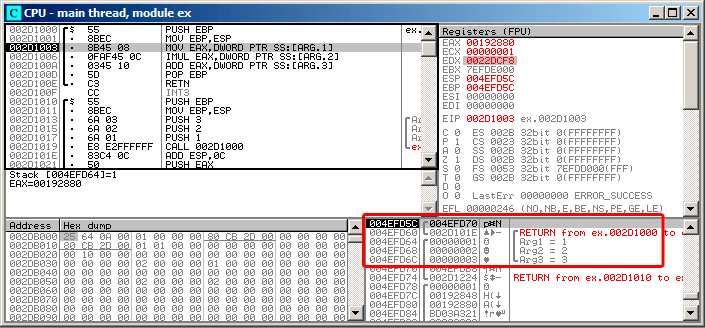
\includegraphics[scale=\FigScale]{patterns/05_passing_arguments/olly.png}
\caption{\olly: \RU{внутри ф-ции}\EN{inside of} \ttf{}\EN{ function}}
\label{fig:passing_arguments_olly}
\end{figure}
\fi

\subsection{GCC}

\RU{Скомпилируем то же в GCC 4.4.1 и посмотрим результат в \IDA:}
\EN{Let's compile the same in GCC 4.4.1 and let's see results in \IDA:}

\lstinputlisting[caption=GCC 4.4.1]{patterns/05_passing_arguments/gcc.asm}

\RU{Практически то же самое, если не считать мелких отличий описанных раннее.}
\EN{Almost the same result.}

\RU{После вызова обоих ф-ций, \glslink{stack pointer}{указатель стека} не возвращается назад, потому что предпоследняя
инструкция}\EN{The \gls{stack pointer} is not returning back after both function exeuction, because penultimate}
\TT{LEAVE} (\ref{x86_ins:LEAVE}) \RU{сделает это за один раз, в конце исполнения}\EN{instruction will do this,
at the end}.


\section{x64}

\index{x86-64}
\RU{В x86-64 всё немного иначе, здесь аргументы функции (4 или 6) передаются через регистры, 
а \gls{callee} из читает их из регистров, а не из стека.}
\EN{The story is a bit different in x86-64. Function arguments (first 4 or first 6 of them) 
are passed in registers i.e. the \gls{callee} reads them from registers instead of reading them from the stack.}

\subsection{MSVC}

\Optimizing MSVC:

\lstinputlisting[caption=\Optimizing MSVC 2012 x64]{patterns/05_passing_arguments/x64_MSVC_Ox.asm.\LANG}

\RU{Как видно, очень компактная функция \ttf берет аргументы прямо из регистров.}
\EN{As we can see, the compact function \ttf takes all its arguments from the registers.}
\RU{Инструкция \LEA используется здесь для сложения чисел. 
Должно быть компилятор посчитал, что это будет эффективнее использования \TT{ADD}.}
\EN{The \LEA instruction here is used for addition,
apparently the compiler considered it faster than \TT{ADD}.}
\index{x86!\Instructions!LEA}
\RU{В самой \main{} \LEA{} также используется для подготовки первого и третьего аргумента: должно быть,
компилятор решил, что \LEA{} будет работать здесь быстрее, чем загрузка значения в регистр при помощи \MOV.}
\EN{\LEA is also used in the \main function to prepare the first and third \ttf arguments. The compiler
must have decided that this would work faster than the usual way of loading values into a register using \MOV instruction.}

\RU{Попробуем посмотреть вывод неоптимизирующего MSVC}\EN{Let's take a look at the non-optimizing MSVC output}:

\lstinputlisting[caption=MSVC 2012 x64]{patterns/05_passing_arguments/x64_MSVC_IDA.asm.\LANG}

\RU{Немного путаннее: все 3 аргумента из регистров зачем-то сохраняются в стеке.}
\EN{It looks somewhat puzzling because all 3 arguments from the registers are saved to the stack for some reason.}
\index{Shadow space}
\label{shadow_space}
\RU{Это называется}\EN{This is called} ``shadow space''
\footnote{\href{http://go.yurichev.com/17256}{MSDN}}: 
\RU{каждая функция в Win64 может (хотя и не обязана) сохранять значения 4-х регистров там.}
\EN{every Win64 may (but is not required to) save all 4 register values there.}
\RU{Это делается по крайней мере из-за двух причин}\EN{This is done for two reasons}: 
1) \RU{в большой функции отвести целый регистр (а тем более 4 регистра) для входного аргумента 
слишком расточительно, так что к нему будет обращение через стек;}
\EN{it is too lavish to allocate a whole register (or even 4 registers) for an input argument,
so it will be accessed via stack;}
2) \RU{отладчик всегда знает, где найти аргументы функции в момент останова}\EN{the debugger is always
aware where to find the function arguments at a break}%
\footnote{\href{http://go.yurichev.com/17257}{MSDN}}.

\RU{Так что, какие-то большие функции могут сохранять входные аргументы в ``shadows space'' 
для использования в будущем, а небольшие функции, как наша, могут этого и не делать.}
\EN{So, some large functions can save their input arguments in the ``shadows space'' if they need to use them
during execution, but some small functions (like ours) may not do this.}

\RU{Место в стеке для ``shadow space'' выделяет именно \gls{caller}.}
\EN{It is a \gls{caller} responsibility to allocate ``shadow space'' in the stack.}

\ifdefined\IncludeGCC
\subsection{GCC}

\Optimizing GCC \RU{также делает понятный код}\EN{generates more or less understandable code}:

\lstinputlisting[caption=\Optimizing GCC 4.4.6 x64]{patterns/05_passing_arguments/x64_GCC_O3.s.\LANG}

\NonOptimizing GCC:

\lstinputlisting[caption=GCC 4.4.6 x64]{patterns/05_passing_arguments/x64_GCC.s.\LANG}

\index{Shadow space}
\RU{В соглашении о вызовах System V *NIX\cite{SysVABI} нет ``shadow space'', но \gls{callee} тоже иногда
должен сохранять где-то аргументы, потому что, опять же, регистров может и не хватить на все действия.
Что мы здесь и видим.}
\EN{There are no ``shadow space'' requirements in System V *NIX\cite{SysVABI}, but the \gls{callee} may need to save
its arguments somewhere in case of registers shortage.}

\subsection{GCC: uint64\_t \RU{вместо}\EN{instead of} int}

\RU{Наш пример работал с 32-битным \Tint, поэтому использовались 32-битные части регистров с префиксом \TT{E-}.}
\EN{Our example works with 32-bit \Tint, that is why 32-bit register parts are used (prefixed by \TT{E-}).}

\RU{Его можно немного переделать, чтобы он заработал с 64-битными значениями}\EN{It can be altered slightly
in order to use 64-bit values}:

\lstinputlisting{patterns/05_passing_arguments/ex64.c}

\lstinputlisting[caption=\Optimizing GCC 4.4.6 x64]{patterns/05_passing_arguments/ex64_GCC_O3_IDA.asm.\LANG}

\RU{Собствено, всё то же самое, только используются регистры \IT{целиком}, с префиксом \TT{R-}.}
\EN{The code is the same, but this time the \IT{full size} registers (prefixed by \TT{R-}) are used.}
\fi

\ifdefined\IncludeARM
\section{ARM}

% subsections
\subsection{\NonOptimizingKeilVI (\ARMMode)}

\begin{lstlisting}
.text:000000A4 00 30 A0 E1                 MOV     R3, R0
.text:000000A8 93 21 20 E0                 MLA     R0, R3, R1, R2
.text:000000AC 1E FF 2F E1                 BX      LR
...
.text:000000B0             main
.text:000000B0 10 40 2D E9                 STMFD   SP!, {R4,LR}
.text:000000B4 03 20 A0 E3                 MOV     R2, #3
.text:000000B8 02 10 A0 E3                 MOV     R1, #2
.text:000000BC 01 00 A0 E3                 MOV     R0, #1
.text:000000C0 F7 FF FF EB                 BL      f
.text:000000C4 00 40 A0 E1                 MOV     R4, R0
.text:000000C8 04 10 A0 E1                 MOV     R1, R4
.text:000000CC 5A 0F 8F E2                 ADR     R0, aD_0        ; "%d\n"
.text:000000D0 E3 18 00 EB                 BL      __2printf
.text:000000D4 00 00 A0 E3                 MOV     R0, #0
.text:000000D8 10 80 BD E8                 LDMFD   SP!, {R4,PC}
\end{lstlisting}

\RU{В функции \main просто вызываются две функции, в первую (\ttf) передается три значения.}
\EN{In function \main, two other functions are called, and three values are passed to the 
first one (\ttf).}

\RU{Как я уже упоминал, первые 4 значения, в ARM обычно передаются в 
первых 4-х регистрах (\Reg{0}-\Reg{3}).}
\EN{As I mentioned before, the first 4 values are usually passed in 
the first 4 registers (\Reg{0}-\Reg{3}) in ARM.}

\EN{The }\RU{Функция }\ttf\RU{, как видно, использует три первых регистра (\Reg{0}-\Reg{2}) как аргументы.}
\EN{function, as it seems, uses the first 3 registers (\Reg{0}-\Reg{2}) as arguments.}

\index{ARM!\Instructions!MLA}
\EN{The }\RU{Инструкция }\TT{MLA} (\IT{Multiply Accumulate}) \RU{перемножает два первых операнда (\Reg{3} и \Reg{1}), 
прибавляет к произведению
третий операнд (\Reg{2}) и помещает результат в нулевой регистр (\Reg{0}), через который, по стандарту, 
возвращаются значения функций.}
\EN{instruction multiplicates its two first operands (\Reg{3} and \Reg{1}), adds the third operand (\Reg{2}) to the product and places
the result into the zeroth register (\Reg{0}), via which, by standard, values are returned from functions.}

\index{Fused multiply–add}
\RU{Умножение и сложение одновременно}\EN{Multiplication and addition at once}\footnote{\WPMAO} 
(\IT{Fused multiply–add}) \RU{это много где применяемая операция, кстати, аналогичной
инструкции в x86 не было до появления FMA-инструкций в SIMD}
\EN{is a very useful operation, by the way, there was no such instruction in x86 
before FMA-instructions appeared in SIMD}
\footnote{\href{http://go.yurichev.com/17103}{wikipedia}}.

\RU{Самая первая инструкция}\EN{The very first} \TT{MOV R3, R0}, \RU{по-видимому, избыточна (можно было бы обойтись только одной инструкцией \TT{MLA})}
\EN{instruction is, apparently, redundant (a single \TT{MLA} instruction could be used here instead)}, 
\RU{компилятор не оптимизировал её, ведь, это компиляция без оптимизации}\EN{the compiler was not optimized it,
since this is non-optimizing compilation}.

\index{ARM!\RU{Переключение режимов}\EN{Mode switching}}
\index{ARM!\Instructions!BX}
\RU{Инструкция \TT{BX} возвращает управление по адресу, записанному в \ac{LR} и, если нужно, 
переключает режимы процессора с thumb на ARM или наоборот.}
\EN{The \TT{BX} instruction returns control to the address stored in the \ac{LR} register and, if necessary, 
switches processor mode from thumb to ARM or vice versa.}
\RU{Это может быть необходимым потому, что, как мы видим, 
функции \ttf неизвестно, из какого кода она будет вызываться, из ARM или thumb.}
\EN{This can be necessary since, as we can see, function \ttf is not aware from what kind of code it may be
called, ARM or thumb.}
\RU{Поэтому, если она будет вызываться из кода thumb, \TT{BX} не только вернет
управление в вызывающую функцию, но также переключит процессор в режим thumb.}
\EN{Thus, if it gets called from thumb code, \TT{BX} will not only return control to the calling function,
but also will switch the processor mode to thumb.}
\RU{Либо не переключит, если функция вызывалась из кода для режима ARM: \cite[A2.3.2]{ARMref}.}
\EN{Or not switch, if the function was called from ARM code \cite[A2.3.2]{ARMref}.}
% look for "BXWritePC()" in manual

\subsection{\OptimizingKeilVI (\ARMMode)}

\begin{lstlisting}[label=ARM_leaf_example1]
.text:00000098             f
.text:00000098 91 20 20 E0                 MLA     R0, R1, R0, R2
.text:0000009C 1E FF 2F E1                 BX      LR
\end{lstlisting}

\myindex{ARM!\Instructions!MLA}
\RU{А вот и функция \ttf, скомпилированная компилятором Keil в режиме полной оптимизации}
\EN{And here is the \ttf function compiled by the Keil compiler in full optimization mode} (\Othree).
\RU{Инструкция \MOV была оптимизирована: теперь \TT{MLA} использует все входящие регистры 
и помещает результат в \Reg{0}, где вызываемая функция будет его читать и использовать.}
\EN{The \MOV instruction was optimized out (or reduced) and now \TT{MLA} uses all 
input registers and also places the result right into \Reg{0},
exactly where the calling function will read and use it.}

\subsection{\OptimizingKeilVI (\ThumbMode)}

\begin{lstlisting}[label=ARM_leaf_example2]
.text:0000005E 48 43                       MULS    R0, R1
.text:00000060 80 18                       ADDS    R0, R0, R2
.text:00000062 70 47                       BX      LR
\end{lstlisting}

\RU{В режиме thumb, инструкция \TT{MLA} недоступна, так что компилятору пришлось сгенерировать код, 
делающий обе операции по отдельности.}
\EN{The \TT{MLA} instruction is not available in thumb mode, so the compiler generates the code doing these two 
operations (multiplication adn addition) separately.}
\index{ARM!\Instructions!MULS}
\index{ARM!\Instructions!ADDS}
\RU{Первая инструкция \TT{MULS} умножает \Reg{0} на \Reg{1} оставляя результат в \Reg{1}.}
\EN{First the \TT{MULS} instruction multiplies \Reg{0} by \Reg{1}, leaving the result in register \Reg{1}.}
\RU{Вторая (\TT{ADDS}) складывает результат и \Reg{2}, оставляя результат в \Reg{0}.}
\EN{The second instruction (\TT{ADDS}) adds the result and \Reg{2} leaving the result in register \Reg{0}.}

\subsection{ARM64}

\subsubsection{\Optimizing GCC (Linaro) 4.9}

\index{Fused multiply–add}
\index{ARM!\Instructions!MADD}
\RU{Тут всё просто}\EN{Everything here is simple}.
\EN{\TT{MADD} is just an instruction doing fused multiply/add (similar to the \TT{MLA} we already saw).}
\RU{\TT{MADD} это просто инструкция, производящая умножение и сложение одновременно (как \TT{MLA}, 
которую мы уже видели).}
\EN{All 3 arguments are passed in the 32-bit parts of X-registers.}
\RU{Все 3 аргумента передаются в 32-битных частях X-регистров.}
\EN{Indeed, the argument types are 32-bit \IT{int}'s.}
\RU{Действительно, типы аргументов это 32-битные \IT{int}'ы.}
\EN{The result is returned in \TT{W0}.}
\RU{Результат возвращается в \TT{W0}.}

\lstinputlisting[caption=\Optimizing GCC (Linaro) 4.9]{patterns/05_passing_arguments/ARM/ARM64_O3.s.\LANG}

\EN{Let's also extend all data types to 64-bit \TT{uint64\_t} and test:}%
\RU{Также расширим все типы данных до 64-битных \TT{uint64\_t} и попробуем:}

\lstinputlisting{patterns/05_passing_arguments/ex64.c}

\begin{lstlisting}
f:
	madd	x0, x0, x1, x2
	ret
main:
	mov	x1, 13396
	adrp	x0, .LC8
	stp	x29, x30, [sp, -16]!
	movk	x1, 0x27d0, lsl 16
	add	x0, x0, :lo12:.LC8
	movk	x1, 0x122, lsl 32
	add	x29, sp, 0
	movk	x1, 0x58be, lsl 48
	bl	printf
	mov	w0, 0
	ldp	x29, x30, [sp], 16
	ret

.LC8:
	.string	"%lld\n"
\end{lstlisting}

\EN{The \ttf{} function is the same, only the whole 64-bit X-registers are now used.}%
\RU{Функция \ttf{} точно такая же, только теперь используются полные части 64-битных X-регистров.}
\RU{Длинные 64-битные значения загружаются в регистры по частям, это описано здесь}%
\EN{Long 64-bit values are loaded into the registers by parts, this is also described here}: \myref{ARM_big_constants_loading}.

\subsubsection{\NonOptimizing GCC (Linaro) 4.9}

\EN{The non-optimizing compiler is more redundant:}
\RU{Неоптимизирующий компилятор выдает немного лишнего кода:}

\begin{lstlisting}
f:
	sub	sp, sp, #16
	str	w0, [sp,12]
	str	w1, [sp,8]
	str	w2, [sp,4]
	ldr	w1, [sp,12]
	ldr	w0, [sp,8]
	mul	w1, w1, w0
	ldr	w0, [sp,4]
	add	w0, w1, w0
	add	sp, sp, 16
	ret
\end{lstlisting}

\EN{The code saves its input arguments in the local stack, 
in case someone (or something) in this function needs using the \TT{W0...W2} 
registers. This prevents overwriting the original
function arguments, which may be needed again in the future.}
\RU{Код сохраняет входные аргументы в локальном стеке на случай если кому-то (или чему-то) в этой функции
понадобится использовать регистры \TT{W0...W2}, перезаписывая оригинальные аргументы функции, которые
могут понадобится в будущем.}
\RU{Это называется}\EN{This is called} \IT{Register Save Area.} \cite{ARM64_PCS}
\RU{Вызываемая функция не обязана сохранять их.}\EN{ The callee, however, is not obliged to save them.}
\RU{Это то же что и}\EN{This is somewhat similar to} \q{Shadow Space}: \myref{shadow_space}.

\RU{Почему оптимизирующий GCC 4.9 убрал этот, сохраняющий аргументы, код?}
\EN{Why did the optimizing GCC 4.9 drop this argument saving code?}
\EN{Because it did some additional optimizing work and concluded
that the function arguments will not be needed in the future 
and also that the registers \TT{W0...W2} will not be used.}
\RU{Потому что он провел дополнительную работу по оптимизации и сделал вывод, 
что аргументы функции не понадобятся в будущем и регистры \TT{W0...W2} также не будут использоваться.}

\index{ARM!\Instructions!MUL}
\index{ARM!\Instructions!ADD}
\RU{Также мы видим пару инструкций \TT{MUL}/\TT{ADD} вместо одной \TT{MADD}.}
\EN{We also see a \TT{MUL}/\TT{ADD} instruction pair instead of single a \TT{MADD}.}


\fi
\ifdefined\IncludeMIPS
\section{MIPS}

\lstinputlisting[caption=\Optimizing GCC 4.4.5]{patterns/05_passing_arguments/MIPS_O3_IDA.lst}

\RU{Первые 4 аргумента ф-ции передаются в четырех регистрах с префиксами A-.}
\EN{First four function arguments are passed in four registers prefixed by A-.}

\index{MIPS!\Instructions!MULT}
\RU{В MIPS есть два специальных регистра: HI и LO, которые выставляются в 64-битный результат умножения
во время исполнения инструцкии \TT{MULT}.}
\EN{There are two special registers in MIPS: HI and LO which are filled by 64-bit result of multiplication while
execution of \TT{MULT} instruction.}
\index{MIPS!\Instructions!MFLO}
\index{MIPS!\Instructions!MFHI}
\RU{К регистрам можно обращаться только используя инструкции \TT{MFLO} и \TT{MFHI}.}
\EN{Registers are accessible only using \TT{MFLO} and \TT{MFHI} instructions.}
\RU{Здесь, \TT{MFLO} берет младшую часть результата умножения и записывает в \$V0.}
\EN{\TT{MFLO} here is taking low-part of result of multiplication and putting it into \$V0.}

\RU{Так что старшая 32-битная часть результата игнорируется (содержимое регистра HI не используется).}
\EN{So high 32-bit part of multiplication result is dropped (contents of HI register is not used).}
\RU{Действительно: мы ведь работаем с 32-битным типом \Tint.}
\EN{Indeed: we work with 32-bit \Tint data type here.}

\index{MIPS!\Instructions!ADDU}
\RU{И наконец, \TT{ADDU} (``Add Unsigned'') прибавляет значение третьего аргумента к результату.}
\EN{Finally, \TT{ADDU} (``Add Unsigned'') adds value of the third argument to the result.}

\index{MIPS!\Instructions!ADD}
\index{MIPS!\Instructions!ADDU}
\index{Ada}
\index{Integer overflow}
\RU{В MIPS есть две разных инструкции сложения:}
\EN{There are two different addition instructions in MIPS:} \TT{ADD} \AndENRU \TT{ADDU}.
\RU{На самом деле, дело не в знаковых числах, но в исключениях: \TT{ADD} может вызвать исключение
во время переполнения, а это иногда полезно\footnote{\url{http://blog.regehr.org/archives/1154}} и поддерживается,
например, в \ac{PL} Ada.}
\EN{In fact, it's not about signedness, but about exceptions: \TT{ADD} can raise exception on overflow,
which is sometimes useful\footnote{\url{http://blog.regehr.org/archives/1154}} and supported in Ada \ac{PL}, 
for instance.}
\TT{ADDU} \RU{не вызывает исключения во время переполнения}\EN{do not raise exceptions on overflow}.
\RU{А так как \CCpp не поддерживает всё это, мы видим здесь \TT{ADDU} вместо \TT{ADD}.}
\EN{Since, \CCpp doesn't support this, here we see \TT{ADDU} instead of \TT{ADD}.}

\RU{32-битный результат оставляется в}\EN{32-bit result is leaved in} \$V0.

\index{MIPS!\Instructions!JAL}
\index{MIPS!\Instructions!JALR}
\RU{В \main есть новая для нас инструкция:}
\EN{There are new instruction for us in \main:} \TT{JAL} (``Jump and Link''). 
\RU{Разница между JAL и JALR в том что относительное смещение кодируется в первой инструкции,
а JALR переходит по абсолютному адресу записанному в регистр (``Jump and Link Register'').}
\EN{Difference between JAL and JALR is that relative offset is encoded in first instruction, 
while JALR jumping to the absolute address stored in register (``Jump and Link Register'').}
\RU{Обе ф-ции \ttf и \main расположены в одном объектном файле, так что относительный адрес
\ttf известен и фиксирован.}
\EN{Both \ttf and \main functions are located in the same object file, so relative address of \ttf 
is known and fixed.}

\fi
